\documentclass[9pt]{beamer}
\mode<presentation>
{
	\usetheme{Warsaw}
	\usecolortheme{beaver}
}

\usepackage[english]{babel}
\usepackage[utf8]{inputenc}
\usepackage[T1]{fontenc}
\usepackage{times}
\usepackage{media9}
\usepackage{color}
\usepackage{physics}
\usepackage{amsmath}
\usepackage{amsfonts}


\newtheorem*{remark}{Remark}

\title[\color{white}{Project N°2}]{A HIGH-ORDER DISCONTINUOUS GALERKIN METHOD FOR THE BIDOMAIN PROBLEM OF CARDIAC ELECTROPHYSIOLOGY}
\subtitle{Project N$^\circ$ 2}
\author[]{\small{\textit{Supervisors: Christian Vergara, Paola Antonietti}}\\ \vspace{4mm} Federica Botta, Matteo Calafà}
\institute[Politecnico di Milano]{\scriptsize{Course of Numerical Analysis for Partial Differential Equations}}
\date{\tiny{A.Y. 2020/2021}}


\logo{
\includegraphics[height=0.5cm]{logo_polimi.png}}



\begin{document}

\frame{\titlepage}

\begin{frame}
\frametitle{Table of Contents}
\tableofcontents
\end{frame}

\begin{frame}
\section{Introduction}
\frametitle{The physical problem}
\begin{center}
Mechanical contraction of the human heart\\

$\uparrow$

Electrical activation of the cardiac cells\\

$\downarrow$

Continuous electrical diffusion over the entire cardiac surface.\\
\end{center}
\begin{columns}
            \begin{column}{0.5\textwidth}
                  \begin{figure}[t]
                  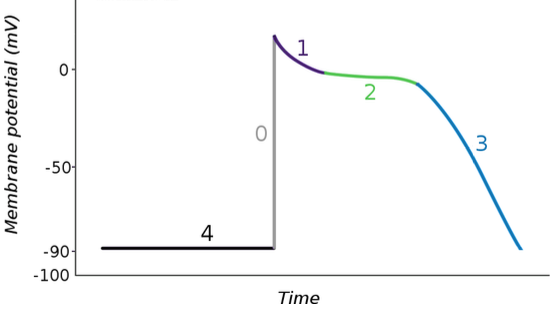
\includegraphics[width = 0.8\textwidth]{./potential_cycle.png}
                  \centering
                  \end{figure}
            \end{column}
            \begin{column}{0.5\textwidth}  
            %\begin{figure}[t]
            %      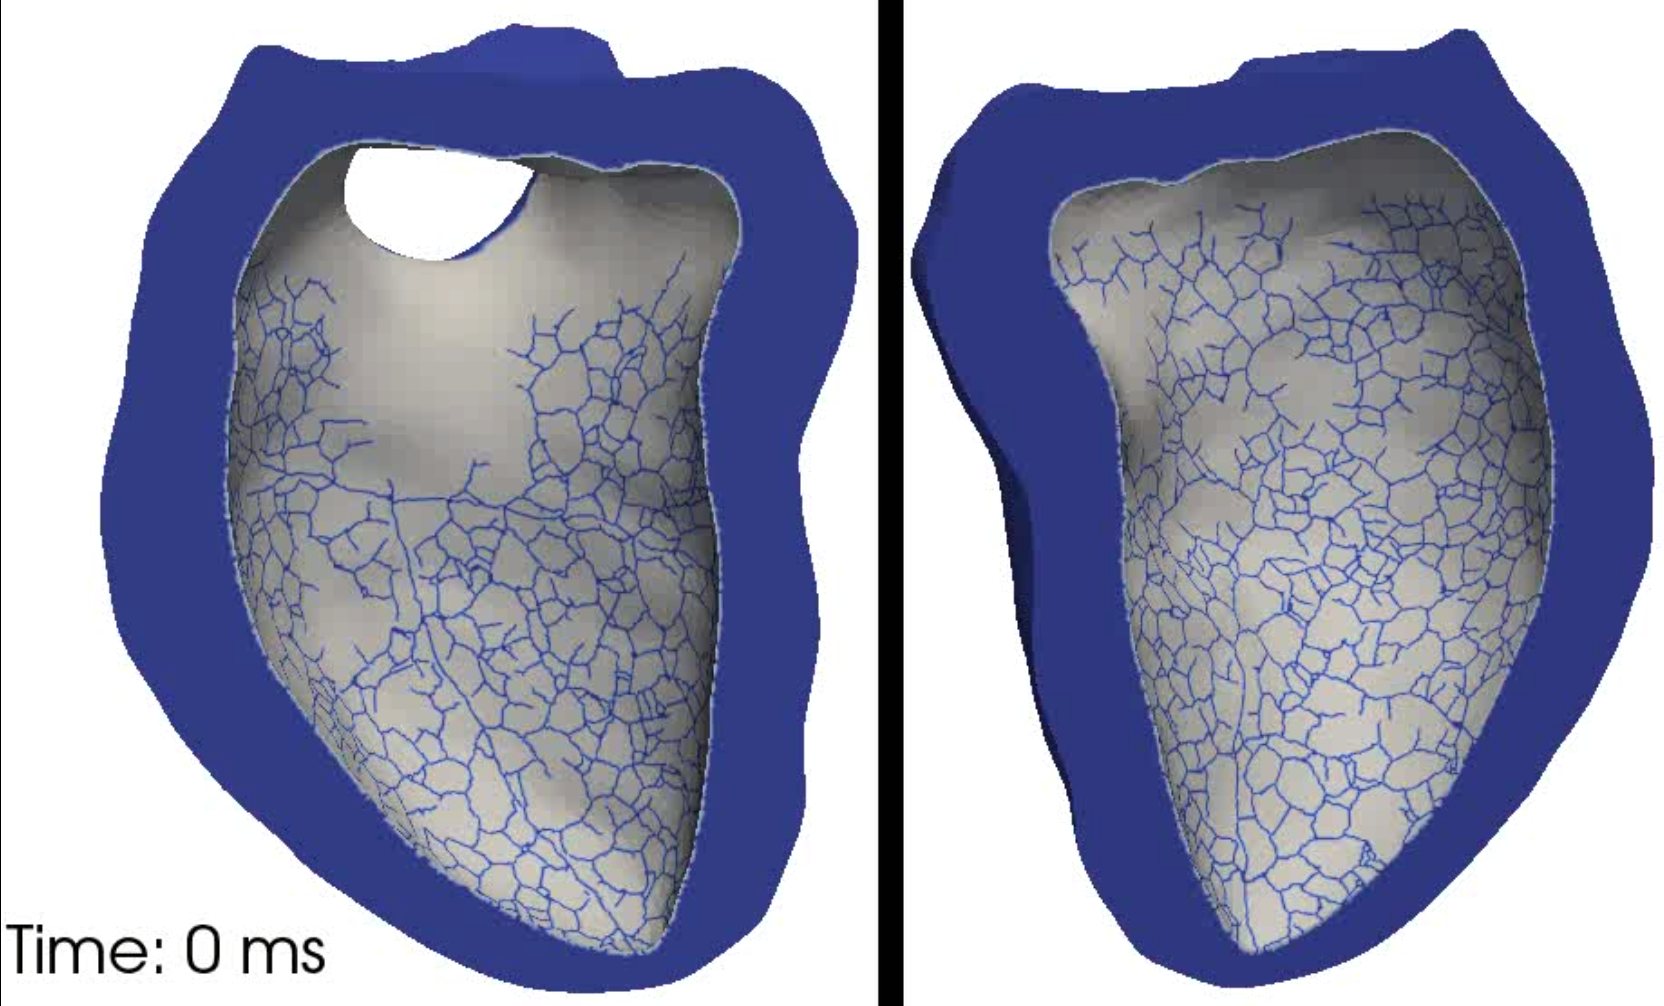
\includegraphics[width = 0.8\textwidth]{./image.png}
            %      \centering
            %      \end{figure} 
                  \includemedia[width=5cm,height=3cm,addresource=Video_Presentazione.mp4,activate=pageopen, flashvars={
                  	source=Video_Presentazione.mp4 &loop=true
                  }]{}{VPlayer.swf}
                  \centering
            \end{column}
     \end{columns}
\end{frame}


\begin{frame}
\frametitle{The mathematical model}
\center
\underline{Bidomain model + FitzHugh-Nagumo with Neumann B.C.}
\begin{equation*}
\small
\begin{cases}
\chi_m C_m\pdv{V_m}{t} - \nabla \cdot (\Sigma_i \nabla \phi_i) + \chi_m I_{ion}(V_m,w) = I_i^{ext},    & \text{in } \Omega_{mus} \cross (0,T],
\\
-\chi_m C_m\pdv{V_m}{t} - \nabla \cdot (\Sigma_e \nabla \phi_e) - \chi_m I_{ion}(V_m,w) = -I_e^{ext},    & \text{in } \Omega_{mus} \cross (0,T],
\\
I_{ion}(V_m,w)=kV_m(V_m-a)(V_m-1)+w, & \text{in } \Omega_{mus} \cross (0,T],
\\
\pdv{w}{t} = \epsilon(V_m-\gamma w),  & \text{in } \Omega_{mus} \cross (0,T],
\\
\Sigma_i\nabla \phi_i \cdot n = b_i,   & \text{on } \partial \Omega_{mus} \cross (0,T],
\\
\Sigma_e\nabla \phi_e \cdot n = b_e,   & \text{on } \partial \Omega_{mus} \cross (0,T],
\\
\text{Initial conditions for } \phi_i,\phi_e, w, & \text{in } \Omega_{mus}\cross\{t=0\}.
\end{cases}
\end{equation*}
\center \small
Unknowns: $\phi_i,\,\phi_e,\, V_m=\phi_i-\phi_e,\, w$
\end{frame}


\begin{frame}
\frametitle{Our objectives}

What had already been done:
\begin{itemize}
	\item Implementation of a Discontinuous Galerkin with FEM basis for the Bidomain problem.
	\item Implementation of a Semi-Implicit temporal scheme.
\end{itemize} \vspace{2mm}
What we did:
\begin{itemize}
	\item Implementation of a Discontinuous Galerkin with \textbf{Dubiner} basis for the Bidomain problem.
	\item Implementation of further temporal schemes.
	\item Bugs corrections and optimizations.
	\item Pseudo-realistic simulations.
\end{itemize}
\end{frame}


\begin{frame}
\section{Dubiner basis implementation}
\frametitle{Analytical definition}
\begin{definition}[Dubiner basis] \label{dubiner}
	The Dubiner basis that generates the space $\mathbb{P}^p(\hat{K})$ of polynomials of degree $p$ over the reference triangle is the set of functions:
	\begin{equation*}
	\begin{gathered}
	 \phi_{ij}: \hat{K} \rightarrow \mathbb{R}, \\
	\phi_{ij}(\xi,\eta) =c_{ij} \, 2^j (1-\eta)^j J_i^{0,0}(\frac{2\xi}{1-\eta}-1) J_j^{2i+1,0} (2\eta-1),
	\end{gathered}
	\end{equation*}
	\vspace{2mm} \\
	\center
	for $i,j=0,\dots,p$ and $i+j \le p$, where $c_{ij} := \sqrt{\frac{2(2i+1)(i+j+1)}{4^i}}$ \\
	and $J_i^{\alpha,\beta}(\cdot)$ is the i-th Jacobi polynomial.
\end{definition}
\end{frame}

\begin{frame}
\frametitle{Properties}
\begin{itemize}
	\item They consist in a pseudo tensor-product of Jacobi polynomials if the following transformation is then applied:
	\begin{columns}
		\begin{column}{0.5\textwidth}
			\begin{equation*}\label{transformation_formula}
			\quad \quad \quad \xi=\frac{(1+a)(1-b)}{4},  \eta=\frac{(1+b)}{2}.
			\end{equation*}
		\end{column}
		\begin{column}{0.5\textwidth}  
			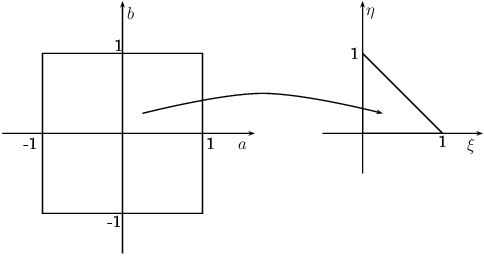
\includegraphics[width = 4cm]{./transformation.png}
		\end{column}
	\end{columns}
    \item They are $L^2(\hat{K})$ orthonormal ($\hat{K}$ is the reference triangle).
\end{itemize}
\end{frame}


\begin{frame}
\frametitle{Main works}
\begin{remark}
	Dubiner basis coefficients of a discretized function have \textbf{modal} meaning instead of a \emph{nodal} meaning.
\end{remark}
Then, our main works regarded:
\begin{itemize}
	\item Methods for the evaluation of the Dubiner functions and gradients in the reference points.
	\item Methods for the evaluation of the FEM coefficients of a discretized function starting from its Dubiner coefficients and viceversa.
	\begin{enumerate}
		\item FEM $\rightarrow$ Dubiner is needed when we use the initial solution data into the Dubiner system.
		\item FEM $\leftarrow$ Dubiner is needed when we want to get the solution obtained from the Dubiner system in a comprehensible form. 
	\end{enumerate}
\end{itemize}
\end{frame}


\begin{frame}
\frametitle{FEM-Dubiner conversion strategies}
Consider:
\begin{itemize}
	\small
	\item An element $\mathcal{K}\in \tau_h$
	\item $\{\psi_{i}\}_{i=1}^{p}$,$\{\varphi_{j}\}_{j=1}^{q}$ as the FEM and Dubiner functions with support in $\mathcal{K}$. 
	\item $\{\hat{u}_i\}_{i=1}^p$,$\{\tilde{u}_j\}_{j=1}^q$ as the FEM and Dubiner coefficients of a function $u_h$.
\end{itemize} \vspace{4mm}
\textbf{FEM $\leftarrow$ Dubiner} \\
Exploiting the nodal meaning of FEM, we compute its value in a point:
\begin{equation*} \label{ref3}
\hat{u}_i = \sum_{j=1}^q \tilde{u}_j\phi_j(x_i),
\end{equation*}
\textbf{FEM $\rightarrow$ Dubiner} \\
Exploiting the $L^2$-orthonormality of Dubiner, we compute its Fourier coeff.:
\begin{equation*}\label{ref4}
\tilde{u}_j = \int_\mathcal{K} u_h(x) \varphi_j(x) \,dx = \int_{\mathcal{K}} \sum_{i=1}^p \hat{u}_i\psi_i(x) \varphi_j(x) \,dx = \sum_{i=1}^p \Big(\int_{\mathcal{K}}\psi_i(x)\varphi_j(x)\,dx \Big) \hat{u}_i.
\end{equation*}
\end{frame}

\end{document}
